\subsection{User Classification}
\textbf{Student Name: Joelian Samuel }Name \textbf{ID:} 0872415\\
This subsection contains the explanation for query by example feature which was build using classification and clustering techniques.
\subsubsection*{Motivation}
Having a search engine for determine user similarity is an interesting feature for a social media. The similarities can be found from the topic of interest, gender, location, hobby, job  or relationship status for example. For this task, the motivation is to classify user data using Google+ user's attribute into several classes and used this classification model to get friends recommendation for other user. 
\subsubsection*{Problem formulation}
Having a set of user data, we should be able to determine what data mining technique is appropriate to classify user and also to build a class model for this data.  
\subsubsection*{Approach}
Since user data don't have any predefined class, we should use clustering technique in order to get the class for each user. Broadly speaking, there are four sub-processes to be undertaken to achieve the objective of this task. Figure~\ref{fig:usercluster} shows us the connection between sub process.
\begin{figure}[H]
	\centering
	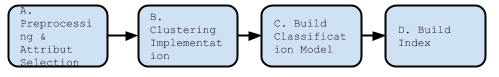
\includegraphics[scale=0.7]{images/usercluster.png}
	\caption{User Clustering Process Flow}
	\label{fig:usercluster}
\end{figure}

A. Pre processing \& Attribute Selection \\
Google+ provides its users with many attributes. However, some users don’t use them. In fact, there are  few users that don’t use any of these attributes at all. Therefore, as a first step of this task, we decided to use two most used attributes : Gender and Relationship Status, also we used one attribute to get user interests : About Me.  \\

For “About Me” attribute, we did a weighting for each word using TF-IDF technique. After we got TF-IDF score for each word, we picked 77 words that have the highest value assuming that words were spread evenly over our data set. These words would represent the interest of user so we called it “Interest Words”. After this process, every user would have 79 attributes. In order to determine a value for every “Interest Words”, we did a simple scanning through every user’s About Me attribute and check whether it contained one of the “Interest words”.  if so, we gave score 1 and 0 otherwise and this was the end of this sub process.  After this process, we would have a new dataset of users with 79 attributes each.  \\

B. Clustering Implementation \\
The new set data of user from sub process A would be used in this sub process. We choose K-Means technique for this part since it was the simplest clustering technique. K means aims is to cluster n data into k clusters in which every data belongs to cluster with the nearest mean. For this task, we used WEKA tools and the parameters that we used are :\\
\begin{enumerate}
	\item Distance Function = Euclidean Distance
	\item Maximum Iteration = 100
	\item Num Cluster       = 15
	\item Seed              = 100
\end{enumerate}
After this process, every user data would be completed with cluster data.  Table~\ref{percentageuser} shows  distribution every cluster. \\
\begin{table}[H]
 \centering
    \begin{tabular}{|l|l|l|l|l|l|}
    \hline
    Cluster & Percentage  & Cluster & Percentage & Cluster & Percentage  \\ \hline
    0       & 153 ( 2 \%)  & 1       & 353 (5 \%)  & 2       & 4674 (64 \%) \\ \hline
    3       & 7 ( 0 \% )   & 4       & 341 (5 \%)  & 5       & 275 (4 \%)   \\ \hline
    6       & 50 ( 1 \%)   & 7       & 20 (0 \%)   & 8       & 35 (0 \%)    \\ \hline
    9       & 842 (12 \%)  & 10      & 53 (1 \%)   & 11      & 31 (0 \%)    \\ \hline
    12      & 114 ( 2 \%)  & 13      & 90 (1 \%)   & 14      & 235 (3 \%)   \\ \hline
    \end{tabular}
    \caption {Summary of Class}
    \label{percentageuser}
\end{table}
The complete result for this process can be seen in Appendix. \\

C. Build Classification Model\\
After sub process B, we again get a new data set. We want to build class model using classification technique so that any new user can be classified into certain class using this model and the technique that we choose was Random Tree. Random Tree is a way to form decision tree by choosing random edge weights. This task also is done by WEKA tools and level of accuracy by using this technique achieves 94.8 \%. The complete result for this process can be seen in Appendix. \\

D. Create Index\\
To improve search performance, the user data is indexed using Apache Lucene.\\


\subsubsection*{Evaluation}
Evaluation is done manually by trying to give a new user input that does not exist in the raw data and the system checks to see if the class that assigned to new user is match with the characteristics of the user. Some examples of data evaluation can be seen in Appendix.
